\documentclass[11pt]{article}
\usepackage{graphicx}
\usepackage{amsmath}
\usepackage{amssymb}
\usepackage{mathtools}
\usepackage{amsthm}
\usepackage{geometry}
\usepackage{xcolor}
\usepackage{booktabs}
\usepackage{hyperref}
\hypersetup{colorlinks=true, linkcolor=blue!55!black, citecolor=blue!55!black,
  urlcolor=blue!55!black}
\geometry{margin=0.9in}
\setlength{\parindent}{0pt}
\setlength{\parskip}{0.55em}

% ---- self-contained macros (distinct names; NOT \input from a sibling) ----
\newcommand{\pzeta}{\zeta}
\newcommand{\gv}[1]{g(#1)}
\newcommand{\pE}{\mathbb{E}}
\newcommand{\pCov}{\mathrm{Cov}}
\newcommand{\RR}{\mathbb{R}}
\newcommand{\pplane}{\mathcal{P}}
\newcommand{\rone}{r_1}
\newcommand{\pmnat}{\,\text{mnat}}
\newcommand{\pud}{u_d}
\newcommand{\ceword}{\mathrm{CE}}
\newcommand{\proj}{\mathrm{proj}}
\newcommand{\Nd}{N_d}
\DeclareMathOperator{\softmax}{softmax}
\newcommand{\keypoint}[1]{%
  \begin{center}\fbox{\parbox{0.93\textwidth}{#1}}\end{center}}
\newcommand{\fool}[1]{\par\smallskip\noindent%
  \textbf{\textcolor{red!60!black}{What would fool you.}}~#1\par\smallskip}

\title{FRA in the constrained-belief world,\\ by worked example}
\author{FRA constrained-belief sprint (Phase 1 complete; Phase 2 partial)}
\date{16 July 2026}

\begin{document}
\maketitle

\begin{abstract}
This is the example-first companion to the formal note
(\texttt{fra\_cbu\_note.tex}). It re-derives the same conclusions about
feature-resolved attention (FRA) --- which attention edits are gauge, which
obey a path calculus --- but it does so from the concrete numbers of
\emph{our own trained models}, one worked arithmetic example at a time, and
only then writes down the general formula each example instantiates. The
setting is paper P2's single-Mess3 one-layer transformer
(\texttt{code/phase1}); every Phase-1 number here is computed \emph{exactly}
by enumerating all $3^{10}=59049$ length-10 sequences with their exact
process probabilities, so there are no error bars unless one is named. Read
it with a Python session open: each section is (i) a concrete question, (ii)
a worked numerical example from a checkpoint we actually trained, (iii) the
general formula it instantiates, and (iv) the mistake you would make if you
skipped the theory. Where our own runs missed a prediction, the miss is in
the text, not hidden.
\end{abstract}

\tableofcontents

\section{The world in 9.4 millinats}\label{sec:world}

\subsection{The question}

Everything below is about one transformer trained on one data process. Before
we can ask what an attention edit \emph{does}, we have to know how much there
was to do in the first place. So: how hard is this task, in nats, and what
exactly must the network compute to solve it?

\subsection{The process, and the one object that runs the whole note}

The data is a single \textbf{Mess3} hidden-Markov process (P2 App.~B; our
\texttt{mess3.py}), with $3$ hidden states and $3$ emitted symbols. Two knobs:
a transition scale $x$ and an emission concentration $a$. We take
\textbf{Config A}: $x=0.15$, $a=0.60$. The marginal hidden transition
$T=(1-2x)I + x(\mathbf 1\mathbf1^\top - I)$ has stationary distribution
$\pi=(\tfrac13,\tfrac13,\tfrac13)$ and eigenvalues $\{1,\pzeta,\pzeta\}$ with
\[
  \pzeta \;=\; 1-3x \;=\; 0.55 ,
\]
the doubly-degenerate subleading eigenvalue --- the correlation time of the
process. This single scalar sets the ``how fast does the past decay'' rate
that the whole note keeps returning to.

The one object you must hold in your head is the \textbf{token displacement}
\[
  \gv{z}\;:=\;\pi\,T^{|z}-\pi\;\in\;\RR^3,
  \qquad T^{|z}:=T^{(z)}/P(z),\quad P(z)=\tfrac13,
\]
the nudge that observing symbol $z$ applies to the belief over the next
hidden state. For Config A these are, exactly (\texttt{mess3.py}, and
reproduced in the formal note's check (i) to $1.1\times10^{-16}$):
\[
  \gv{0}=\!\begin{pmatrix}\phantom{-}0.2667\\-0.1333\\-0.1333\end{pmatrix}\!,\quad
  \gv{1}=\!\begin{pmatrix}-0.1333\\\phantom{-}0.2667\\-0.1333\end{pmatrix}\!,\quad
  \gv{2}=\!\begin{pmatrix}-0.1333\\-0.1333\\\phantom{-}0.2667\end{pmatrix}\!.
\]
Three facts about these vectors carry a surprising amount of the story.
Each sums to zero ($\gv{z}\cdot\mathbf 1=0$), so all three live in the
$2$-dimensional \textbf{belief plane}
$\pplane=\{v:\,v\cdot\mathbf1=0\}$. They \emph{also} sum to zero across tokens,
$\sum_z\gv{z}=0$, so any two of them span $\pplane$ and the third is minus their
sum. And they are symmetric: $\|\gv{z}\|$ is the same for all $z$, and no two are
orthogonal ($\gv{z}\cdot\gv{z'}=-\tfrac12\|\gv{z}\|^2$ for $z\ne z'$). Hold onto
``two dimensions, three vectors, summing to zero'' --- in
Section~\ref{sec:ov} it is what makes selective concept removal
\emph{geometrically impossible} in this world.

\subsection{The constrained update: what the transformer must compute}

P2's central claim is that this transformer does not run exact Bayesian
filtering. It runs a linear-in-log-space surrogate, the \textbf{constrained
belief update}. In spectral form (formal note Eq.~(S0.4); \texttt{mess3.py}),
the prediction after reading a length-$d$ prefix $z_{1:d}$ is
\keypoint{%
\textbf{The constrained update.}
\[
  \rone(d)\;=\;\pi+\pud,\qquad
  \pud\;=\;\sum_{s=1}^{d}\pzeta^{\,d-s}\,\gv{z_s}.
\]
Every lag-$(d-s)$ token contributes its displacement $\gv{z_s}$,
\emph{geometrically discounted} by $\pzeta^{\,d-s}$. All the lag structure is
in the scalar $\pzeta^{\,d-s}$; all the token structure is in the plane
vector $\gv{z_s}$. That factorization is the reason FRA has anything clean to
say here.}

\subsection{Worked example: one sequence, by hand}\label{sec:worked-r1}

Take the concrete length-10 sequence
\[
  z_{1:10} \;=\; (0,\,2,\,1,\,0,\,1,\,2,\,2,\,0,\,1,\,0).
\]
Compute $\rone(2)$, the prediction after the first two tokens, by hand. Only
lags $0$ and $1$ exist, so
\[
  u_2 = \pzeta^{1}\gv{0}+\pzeta^{0}\gv{2}
      = 0.55\!\begin{pmatrix}0.2667\\-0.1333\\-0.1333\end{pmatrix}
      +\begin{pmatrix}-0.1333\\-0.1333\\0.2667\end{pmatrix}
      =\begin{pmatrix}0.0133\\-0.2067\\0.1933\end{pmatrix},
\]
so $\rone(2)=\pi+u_2=(0.3467,\,0.1267,\,0.5267)$. Running the exact recursion
in \texttt{mess3.py} on this sequence returns
$(0.34667,\,0.12667,\,0.52667)$ --- identical (we checked all destinations
$d=1,2,3,10$ to $\le 5\times10^{-16}$). The prediction is a $\pi$-anchored
walk in the belief plane, one geometrically-discounted $\gv{z_s}$ kick per
observed token. That is the entire ``computation''; the transformer's job is
to realize this map with attention.

\subsection{The anchors: how many nats are on the table}\label{sec:anchors}

Now the scoreboard. Averaged over query positions with exact process
probabilities (\texttt{train\_log.json}, \texttt{anchors.json}), the
cross-entropies are
\begin{center}
\begin{tabular}{lrl}
\toprule
predictor & CE (nats) & what it is \\
\midrule
unigram $\log 3$ & $1.098612$ & know nothing but the marginal \\
trained model (Config A) & $1.089462$ & our checkpoint, exact enumeration \\
$\rone$-ansatz (clipped readout) & $1.089562$ & the constrained update, read out linearly \\
exact Bayes & $1.089203$ & optimal filtering \\
\bottomrule
\end{tabular}
\end{center}
The distance from ``know nothing'' to ``optimal'' is
$1.098612-1.089203 = 0.009409$ nats $=\mathbf{9.4\pmnat}$. \emph{That is the
entire size of this world.} Every attention edit, every FRA reading, every
gauge swing in this note plays out inside a $9.4$-millinat budget. The trained
model sits $1.089462-1.089203 = 0.259\pmnat$ above Bayes, i.e.\ it captures
$(1.098612-1.089462)/0.009409 = 97.3\%$ of the available information. Notice
also that the trained model (\,$1.089462$\,) actually \emph{beats} the
$\rone$-ansatz readout (\,$1.089562$\,): the network's own MLP readout is a
touch better than clipping the constrained update. (Config A2, a second seed,
lands the other side of the ansatz; the whole seed spread is $\approx
0.25\pmnat$.)

\fool{If you skip this section and dive straight into ``mechanism,'' every
number in the note looks alarmingly small and you will over-read noise. A
$1$-millinat cut effect is not weak evidence of a weak mechanism; it is
\emph{most of a mechanism} in a $9.4$-millinat world. Conversely, a
``structure'' you find that would cost the loss $10^{-5}$ nats to destroy is,
for this task, indistinguishable from nothing. Section~\ref{sec:ladder} makes
the ``indistinguishable from nothing'' floor precise, and it turns out to
swallow most of what FRA-QK will later appear to measure.}

\section{How much is each lag worth?}\label{sec:ladder}

\subsection{The question}

The constrained update sums a contribution from every past token. Before we
attribute anything to how attention routes those contributions, we should ask
the loss which of them it even cares about. If lag $7$ is worth nothing, then
whatever the attention pattern does at lag $7$ is unconstrained, and a ``clean
mechanism'' found there is a fiction the gradient never signed off on.

\begin{figure}[t]
\centering
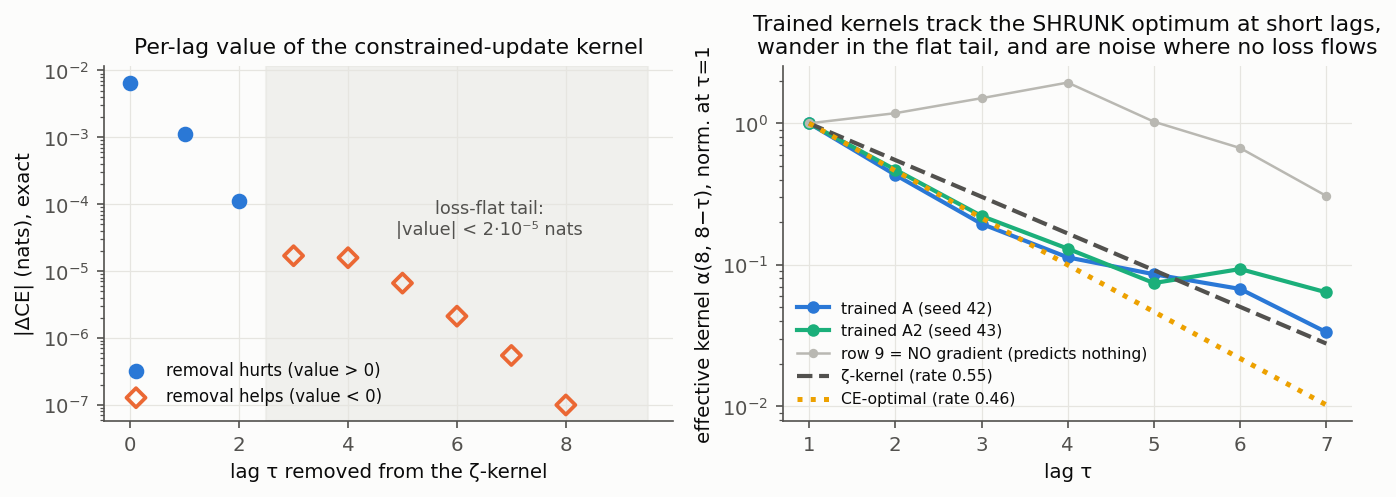
\includegraphics[width=\textwidth]{../figures/kernel_flatness.png}
\caption{\textbf{The value ladder and the trained kernels.} Left: the exact CE
value of each lag $\tau$ (nats it buys), collapsing to a negative
sub-$2\times10^{-5}$ floor beyond $\tau=2$. Right: trained attention kernels by
destination row. Where the loss pins them (lags $1$--$4$) both seeds track the
\emph{shrunk} optimum (ratio $\approx0.43$--$0.45$, below $\pzeta=0.55$); in the
flat tail the seeds wander; the gradient-free last row (gray) is an order of
magnitude off.}
\label{fig:kernel}
\end{figure}

\subsection{Worked example: the exact ladder}

Because Config A is exactly enumerable, we can compute the CE \emph{value of
lag $\tau$}: fit the best kernel that uses lags $0..\tau$, and record how many
nats the $\tau$-th rung buys over stopping at $\tau-1$
(\texttt{kernel\_ce.py}, \texttt{out/kernel\_ce\_A.json}):
\begin{center}
\begin{tabular}{lrrrrrrr}
\toprule
lag $\tau$ & $0$ & $1$ & $2$ & $3$ & $4$ & $5$ & $\ge6$ \\
\midrule
value (mnat) & $6.591$ & $1.106$ & $0.1132$ & $-0.0170$ & $-0.0159$ & $-0.0066$ & $\le -2\times10^{-6}$ \\
\bottomrule
\end{tabular}
\end{center}
Read the ladder. Lag $0$ is worth $6.6\pmnat$, lag $1$ is worth $1.1\pmnat$,
lag $2$ is worth $0.11\pmnat$ --- and \textbf{every lag beyond $2$ has a
\emph{negative} value below $2\times10^{-5}$ nats}. Negative: including it
\emph{hurts}. That sign is not a rounding artifact; it is the tell of
double-counting (next subsection). The first three rungs sum to essentially the
whole $9.4$-millinat budget; the rest of the geometric tail is, to the loss,
noise.

\subsection{The shrinkage surprise, and why the sign flips}

Here is the surprise. The process eigenvalue is $\pzeta=0.55$, so you would
guess the CE-optimal kernel decays at rate $0.55$. It does not. The best
geometric kernel in the $\rone$-family decays at rate
\[
  \rho^\star \;=\; 0.464 \quad(\text{measured ratios } 0.462,\,0.464,\,0.465,\,0.466),
\]
\emph{faster} than the process ($\ceword=1.089316$ vs $\pzeta$-kernel
$1.089562$; and letting the kernel vary freely per destination --- $55$
parameters instead of $10$ --- buys under $\mathbf{3}$ \textbf{micro}nats more,
$1.089316\!\to\!1.089313$). Why does optimal decay undershoot the process
eigenvalue?

\textbf{Worked example (2 correlated regressors; illustrative arithmetic).}
The constrained update weights lag $\tau$ by the \emph{marginal} coupling
$\pzeta^{\tau}$ --- the covariance a single lagged token has with the target if
it were the only evidence. But consecutive tokens are correlated (that is what
$\pzeta$ \emph{is}), so their evidence overlaps, and a sum of marginal weights
counts the overlap twice. Strip it to two predictors $a,b$ of a target $y$,
each with unit target-covariance $\pE[ay]=\pE[by]=1$ and unit variance
$\pE[a^2]=\pE[b^2]=1$, but mutually correlated $\pE[ab]=\pzeta$. Used alone,
each wants coefficient $1$. Used \emph{together}, the normal equations
$\begin{psmallmatrix}1&\pzeta\\\pzeta&1\end{psmallmatrix}
\begin{psmallmatrix}\beta_a\\\beta_b\end{psmallmatrix}=
\begin{psmallmatrix}1\\1\end{psmallmatrix}$ give
\[
  \beta_a=\beta_b=\frac{1}{1+\pzeta}=\frac{1}{1.55}=0.645 ,
\]
each shrunk to $64.5\%$ of its marginal value so the two do not double-count
their shared part. Add a \emph{third} correlated regressor and the shrinkage
compounds, pushing the effective lag-to-lag ratio below $\pzeta$; the exact
constrained-belief version of this partial-regression shrinkage lands the
optimal rate at $0.464$. And once the marginal-weight kernel over-counts,
\emph{adding} another over-counted tail term makes CE worse --- the negative
rungs of the ladder.

The shrinkage is not a CE artifact. Scanning the matched geometric family under
\emph{squared error} instead of cross-entropy gives an MSE-optimal rate of
$0.467$ (\texttt{close\_gaps.json}) --- essentially the same $0.46$, not
$\pzeta=0.55$. CE and MSE agree on the shrunk rate: it is a property of the
correlated evidence, a P3 Toeplitz-optimality echo, not of the particular loss.

\subsection{The trap: the row the gradient never touched}

Now the mistake this section exists to prevent. Config A has context length
$10$; the query at position $t$ (0-based) predicts token $t{+}1$. The last
\emph{scored} query is position $8$ (it predicts token $9$). \textbf{Position
$9$ would predict token $10$, which does not exist} --- so no loss term ever
references destination row $9$, and \emph{no gradient ever flows through it}.
Its attention pattern is initialization noise, frozen.

\textbf{Worked consequence.} If you fit ``the decay rate of the trained
attention kernel'' by pooling all destination rows --- including row $9$ --- you
read a rate of $0.68$--$0.71$, comfortably \emph{above} $\pzeta=0.55$, and you
would conclude the model \emph{contradicts} the spectral ansatz. Restrict to
the rows the loss actually trained (rows $1$--$8$) and the fitted rate is
$0.43$--$0.45$, matching the CE-optimal $0.464$ and cleanly \emph{below}
$\pzeta$ (Fig.~\ref{fig:kernel}, right: the gray gradient-free row sits an order
of magnitude off, with a spurious bump at lag $4$). The pooled fit was
dominated by one row of noise.

\keypoint{\textbf{Moral.} Before reading structure off a trained model, find out
what the loss \emph{pinned}. In this world that is: lag $0$, most of lag $1$, a
sliver of lag $2$, and rows $1$--$8$. Everything else --- the geometric tail,
row $9$ --- is loss-flat, and any FRA attribution placed there is reading seed
noise dressed as mechanism. This one fact ($\tau\ge3$ and row $9$ are free) will
explain, in Section~\ref{sec:dial}, why the FRA-QK ``removal'' effect can be
dialed across a $140\times$ range without the loss noticing.}

\fool{The two decoys here are opposite in sign. The loss-flat \emph{tail}
tempts you to interpret wiggles that cost microNats to erase; the untrained
\emph{row} tempts you to interpret a rate that is pure initialization. Both
look like ``the model does something interesting at long range.'' Neither
survives asking the loss.}

\section{The dial: what FRA-QK actually measures}\label{sec:dial}

\subsection{The question}

FRA-QK decomposes each attention \emph{score} into feature$\times$feature
pieces and asks which token-pair terms drive who-attends-to-whom. In this
world the token-pair terms carry a real $\approx10\%$ of the score mass. So:
cut them, and how much does the model's behavior change?

\subsection{The four score blocks}

Write the residual at a position as token feature plus positional feature,
$x_s=e(z_s)+p_s$, and split query and key the same way,
$q_d=q_E(z_d)+q_P(d)$, $k_s=k_E(z_s)+k_P(s)$. The score is bilinear, so it
splits into \emph{four} blocks (formal note Eq.~(S2.2)):
\[
  \sigma(d,s)=
  \underbrace{q_P(d)\!\cdot\!k_P(s)}_{\text{pos}\times\text{pos}}
  +\underbrace{q_P(d)\!\cdot\!k_E(z_s)}_{\text{pos}\times\text{tok}}
  +\underbrace{q_E(z_d)\!\cdot\!k_P(s)}_{\text{tok}\times\text{pos}}
  +\underbrace{q_E(z_d)\!\cdot\!k_E(z_s)}_{\text{tok}\times\text{tok}\,=\,Q(z_d,z_s)}.
\]
FRA-QK's ``feature$\times$feature score mass'' is the last block $Q$. In our
Config A checkpoint it is about $10\%$ of the pattern-weighted score budget
(\texttt{gauge\_qk.json}, \texttt{tok\_tok\_share} $\approx 0.10$ across the
whole dial below). Ten percent is not nothing, and the naive attribution logic
says: cut it and the routing should move.

\subsection{One softmax row, and why a cut is a tilt}

The reason it will \emph{not} move is one identity. A row of attention is a
probability distribution $A_s=e^{\sigma_s}/\sum_{s'}e^{\sigma_{s'}}$ over keys,
and the head output is the expectation $c_d=\sum_s A_s v_s=\pE_A[v]$. Any score
edit is $\sigma\to\sigma-c\,\delta$, and its first-order effect on the output is
\emph{a covariance across the row}:
\[
  \Delta c_d \;=\; -\,c\,\pCov_A(\delta,\,v)\;+\;O(c^2\,\mathrm{osc}(\delta)^2).
\]
So an edit moves the output only insofar as $\delta$ \emph{covaries with the
values} $v$ down the row. Two consequences drive everything below: (a) an edit
that is \emph{constant across keys} does exactly nothing (softmax kills row
constants); (b) the magnitude of a token cut is set by whatever scalar
multiplies the indicator $\mathbb 1[z_s=z^*]$ in $\delta$. For a key-side cut of
token $z^*$ that scalar is the same for every token --- the \textbf{pedestal}
$\beta(d)=q_d\cdot\bar k_E$ (formal note Eq.~(S2.5)). Cut effect
$\propto\beta$. Keep that.

\subsection{Worked example: dialing the pedestal to zero}\label{sec:g1}

\begin{figure}[t]
\centering

\includegraphics[width=0.86\textwidth]{../figures/gauge_dial.png}
\caption{\textbf{The G1 gauge dial.} As the embedding/position re-split
parameter $t$ sweeps, every logit is unchanged (max difference $\sim
7\times10^{-7}$), yet the \emph{named} operation ``cut token 0's key-side
FRA-QK term at gain 1'' swings its $\Delta\ceword$ over $140\times$, minimized
exactly where the measured pedestal $\beta$ crosses zero.}
\label{fig:gauge}
\end{figure}

Here is the whole point of FRA-QK in one experiment. There is a
\emph{loss-preserving reparameterization} --- gauge move G1 --- that moves
token content into positions and back: $e(z)\to e(z)+t\,u$ with every position
absorbing $-t\,u$. Because $x_s=e(z_s)+p_s$ is unchanged, \textbf{every
residual, activation, and logit is bit-identical} along the entire dial: we
measured the max logit difference at $\sim7\times10^{-7}$ (float32 roundoff) for
every $t\in[-1,2]$ (\texttt{gauge\_qk.json}, \texttt{identity\_max\_logit\_diff}).
The model is, forward-pass, the same model at every $t$.

But G1 \emph{does} move where the split puts ``token content,'' so it moves the
pedestal $\beta$, and therefore the FRA-QK cut coefficient. Sweeping $t$ and
recording (i) the per-token pedestal and (ii) the exact-enumeration
$\Delta\ceword$ of the operation ``cut token $0$'s key-side term at gain $1$'':
\begin{center}
\begin{tabular}{lrrrrr}
\toprule
dial $t$ & $-1.0$ & $0.0$ & $\mathbf{1.0}$ & $1.5$ & $2.0$ \\
\midrule
pedestal $\bar\beta$ (mean) & $-0.69$ & $-0.31$ & $\mathbf{+0.07}$ & $+0.26$ & $+0.45$ \\
$\Delta\ceword$ (nats) & $1.1{\times}10^{-3}$ & $2.8{\times}10^{-4}$ &
$\mathbf{8.1{\times}10^{-6}}$ & $5.2{\times}10^{-5}$ & $1.9{\times}10^{-4}$ \\
identity logit diff & $6{\times}10^{-7}$ & $0$ & $6{\times}10^{-7}$ &
$7{\times}10^{-7}$ & $6{\times}10^{-7}$ \\
\bottomrule
\end{tabular}
\end{center}
At $t=0$ the pedestal per token is $-0.287$, $-0.313$, $-0.323$; it crosses zero
at $t\approx1$ (there $+0.036$, $+0.097$, $+0.074$); the $\Delta\ceword$ of the
\emph{same named cut} runs $1.1{\times}10^{-3}$ to $8.1{\times}10^{-6}$ to
$1.9{\times}10^{-4}$, a \textbf{V-shape of range} $\mathbf{138\times}$ whose floor
sits where $\beta\approx0$. The behavior of the model never changed; only the
coordinate did.

The floor itself is telling: $8.1\times10^{-6}$ nats is \emph{below} the
loss-flat scale of Section~\ref{sec:ladder}. The gauge-invariant content of the
FRA-QK cut is indistinguishable from the noise the loss never sees. (Why so
inert at heart? The target kernel $\pzeta^{\,d-s}\gv{z_s}$ is
\emph{separable} --- a lag scalar times a content vector --- so the token-pair
score block carries no causal handle at any minimizer; formal note
Thm.~boundary. Mess3 is on the null side of that boundary.)

\subsection{A corroborating null: cut every token and nothing should happen}

The theory says cutting the \emph{whole} token set on the key side is
\emph{exactly inert}: every key carries one token, so the summed edit is a
per-row constant $\beta(d)$, and constants die in softmax. On the idealized
model this holds to $2\times10^{-16}$. On the \emph{trained} model it does not
quite: the full-token-set cut costs $\Delta\ceword=3.0\times10^{-4}$ at $t=0$,
about the same as a single-token cut ($2.8\times10^{-4}$). The reason is
\emph{content leak}: the trained pattern is not perfectly token-independent
(its premise-violation $\varepsilon$ is $1.5\times$ the positional profile
slope, \texttt{gauge\_qk.json}), so the summed edit is not perfectly constant.
The theory predicts exactly this: an $O(c\varepsilon)$ residue, pure leak. The
``exactly inert'' law is an $\varepsilon\!=\!0$ statement; on a real checkpoint
you see the leak, not zero.

\keypoint{\textbf{Moral.} A number that a loss-preserving reparameterization can
send to zero is a \emph{gauge coordinate}, not a mechanism. The FRA-QK
``token-0 removal effect'' is such a number: same model, same enumeration,
$140\times$ range at bit-identical behavior. Before you report an attention-score
attribution, \emph{dial the gauge} and see whether your effect survives.}

\fool{The $10\%$ ``feature$\times$feature score mass'' is real and it is a
trap. Score mass is not causal mass. Here the entire token-dependent part of the
score block is additively separable into gauge coordinates (formal note
Eq.~(S2.3)), so it can be made to look like $0\%$ or $100\%$ of the mechanism
without touching a single logit. The only invariant --- the centered
interaction $\hat q_E(z)\!\cdot\!\hat k_E(z')$ --- is identically zero in this
world.}

\section{Cutting what flows: FRA-OV is the real handle}\label{sec:ov}

\subsection{The question}

FRA-QK was gauge because it edits \emph{scores}, and scores are one
reparameterization away from anything. FRA-OV edits the attention
\emph{output}: it subtracts the content a token's channel actually transports
into the residual stream. That content is causal. The questions become
quantitative: if we sever token $z^*$'s channel at gain $c$, how far does the
model's belief-tracking fall --- and can we predict the number \emph{before
running a single edited forward pass}?

\begin{figure}[t]
\centering
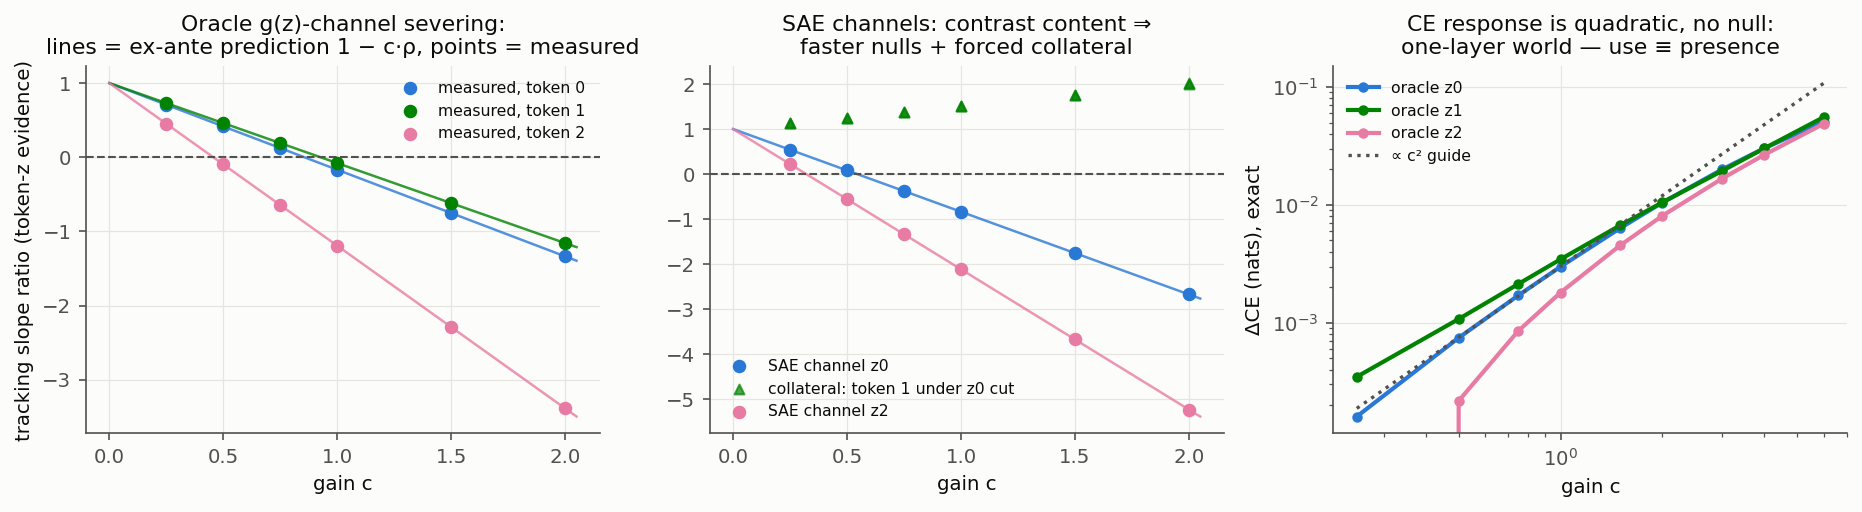
\includegraphics[width=\textwidth]{../figures/ov_control.png}
\caption{\textbf{FRA-OV is causal.} Left: severing a token's channel drops its
belief-tracking \emph{linearly} in the gain $c$, crossing zero at the predicted
null $c^\star=1/\rho_{\mathrm{eff}}$. Middle: geometrically forced collateral ---
severing token 0 \emph{raises} the other tokens' tracking. Right: CE removal is
\emph{quadratic} in $c$ with no behavioral null (slope-2 guide), because a
one-layer model has no redundant path.}
\label{fig:ov}
\end{figure}

\subsection{The attribution, and why it over-carries: the warp}

The per-(token, lag) content the head transports is (formal note
Eq.~(S3.1)) the constrained-update term itself,
$\Delta_{s\to d}=A_{d,s}\,f(v_s)=\pzeta^{\,d-s}\gv{z_s}$. But there is a
subtlety that decides whether ex-ante predictions land: with additive
positional embeddings, the softmax-realizable head output is not $\pud$ but a
\emph{token-independent multiplicative warp} of it (formal note Eq.~(S1.7);
twin's Finding 5),
\[
  f(c_d)=\lambda_d\,\pud,\qquad \lambda_d=\frac{1}{1-\pzeta^{\,d}}\ge 1 .
\]
Worked, for $\pzeta=0.55$:
\[
  \lambda_{1..5}=\bigl(\tfrac{1}{1-0.55},\,\tfrac{1}{1-0.55^2},\,\dots\bigr)
  =(2.22,\;1.43,\;1.20,\;1.10,\;1.05)\longrightarrow 1 .
\]
The head \emph{over}-carries at small $d$ (a normalization overshoot
$\pzeta^d/(1-\pzeta^d)$, largest early), then relaxes to unity. This warp is
one of the two reasons the tracking slope $\rho_{\mathrm{eff}}$ will exceed $1$
below; the other is the CE-shrinkage of Section~\ref{sec:ladder} (the model's
readout, unlike the clipped $\rone$, scales content up).

\subsection{The skip/diagonal split (the \texorpdfstring{$k{=}0$}{k=0} gauge)}

One subtlety before we cut. The current token's own displacement $\gv{z_d}$
(lag 0) reaches the readout by \emph{two} routes: the residual \textbf{skip}
connection, and \textbf{diagonal attention} (position $d$ attending to itself).
Only their sum is pinned; the split is a gauge (the $k{=}0$ degree of freedom).
An OV cut removes only the diagonal share. Measured on the trained model, the
lag-0 $\gv{z}$-projection splits as (\texttt{refine\_rho.json}):
\begin{center}
\begin{tabular}{lrrr}
\toprule
token & diagonal share & skip share & diagonal fraction \\
\midrule
$z_0$ & $0.824$ & $0.142$ & $0.85$ \\
$z_1$ & $0.801$ & $0.148$ & $0.84$ \\
$z_2$ & $0.561$ & $0.249$ & $0.69$ \\
\bottomrule
\end{tabular}
\end{center}
So $\approx 80\%$ of tokens 0 and 1's lag-0 content is on the (cuttable)
diagonal, but only $\approx 69\%$ of token 2's. That asymmetry will show up
again in token 2's numbers. (The rows do not sum to exactly $1$ --- $0.97,
0.95, 0.81$ --- because of the warp and shrinkage above; the shortfall is real,
not rounding.)

\subsection{Worked example: predicting the tracking slope ex ante}\label{sec:rho}

Now the headline. Define the \textbf{tracking slope} $\rho_{\mathrm{eff}}$: as
we sever token $z^*$'s channel at gain $c$, the model's belief coupling to
$z^*$-evidence falls as $1-c\,\rho_{\mathrm{eff}}$. We predict
$\rho_{\mathrm{eff}}$ from \emph{clean-model statistics only} --- no edited
forward passes --- by a covariance recipe (\texttt{refine\_rho.py}):
\[
  \rho_{\mathrm{eff}}\;=\;\frac{J}{E^2\cdot \text{slope}_0},
  \qquad
  J=\Big\langle\!\!\sum_{s\le d:\,z_s=z^*}\!\! A_{d,s}\,\proj_{\gv{z^*}}\!\big(f(v_s)\big)\;,\;\omega_{z^*}(d)\Big\rangle_{\!P},
\]
where $J$ is the (probability-weighted, over all $d$) covariance of the removed
channel's $\gv{z^*}$-projected content with the true evidence
$\omega_{z^*}(d)=\sum_{s\le d:\,z_s=z^*}\pzeta^{\,d-s}$; $E^2=\langle
\omega_{z^*}^2\rangle_P$ is the evidence variance; and $\text{slope}_0$ is the
clean model's belief-tracking slope, which converts the answer into clean-model
units.

Do token $0$, oracle basis, by the numbers (\texttt{refine\_rho.json} fields
\texttt{rho\_absolute\_units\_J\_over\_E2} and \texttt{rho\_eff\_predicted};
\texttt{ov\_edits.json}):
\[
  \frac{J}{E^2}=0.8766,\qquad \text{slope}_0=0.7503,\qquad
  \rho_{\mathrm{eff}}=\frac{0.8766}{0.7503}=\mathbf{1.1683}.
\]
The measured slope, from actually running the edited model over all $3^{10}$
sequences, is $\mathbf{1.1683}$. Not close --- equal to the digits shown. And it
is not a one-off; the same recipe nails all five channels we edited:
\begin{center}
\begin{tabular}{lrrrr}
\toprule
channel & $J/E^2$ & $\text{slope}_0$ & predicted $\rho_{\mathrm{eff}}$ & measured \\
\midrule
oracle $z_0$ & $0.8766$ & $0.7503$ & $1.1683$ & $1.1683$ \\
oracle $z_1$ & $0.9138$ & $0.8470$ & $1.0789$ & $1.0789$ \\
oracle $z_2$ & $0.8114$ & $0.3699$ & $2.1935$ & $2.1935$ \\
SAE $z_0$    & $1.3794$ & $0.7503$ & $1.8384$ & $1.8384$ \\
SAE $z_2$    & $1.1534$ & $0.3699$ & $3.1181$ & $3.1181$ \\
\bottomrule
\end{tabular}
\end{center}
Every row agrees to the four significant figures printed (in fact to
$\sim10^{-7}$; we re-derived the table independently). This is FRA-OV working
exactly as an attribution should: the clean model's own statistics tell you, in
advance, how much a channel carries.

\subsection{The null, for free}

Because tracking falls as $1-c\,\rho_{\mathrm{eff}}$, the \emph{concept-nulling
gain} --- the $c$ at which token $z^*$'s tracking hits zero --- is predicted
before any edit:
\[
  c^\star=\frac{1}{\rho_{\mathrm{eff}}} .
\]
For oracle $z_0$: $c^\star=1/1.1683=\mathbf{0.856}$. Sweep the edited model and
the tracking ratio crosses zero at $c\approx0.856$ (it is $+0.124$ at $c=0.75$,
$-0.168$ at $c=1.0$). Predicted before measured, to three figures. Note
$c^\star<1$: \emph{exact} severing ($c=1$) here \emph{over}-reaches, because the
diagonal share is large (Section above). The folk intuition ``severing always
under-reaches'' is simply false in this world.

\subsection{Collateral is geometrically forced}

Look at the middle panel of Fig.~\ref{fig:ov}. Sever token $0$ and the
\emph{other} tokens' tracking \emph{rises}: at $c=1$, token 1's tracking ratio
has climbed to $1.17\times$ and token 2's to $1.39\times$ while token 0's has
been driven to $-0.17$. This is not a leak or a method flaw. It is forced by the
geometry of Section~\ref{sec:world}: the three displacements $\gv{0},\gv{1},\gv{2}$
live in a $2$-dimensional plane and sum to zero, so \emph{no two are
orthogonal} and no single direction is orthogonal to the other two. Pushing the
belief's $\gv{0}$-component down necessarily moves its $\gv{1}$- and
$\gv{2}$-components (each $\gv{z}$ has a nonzero $\gv{0}$-projection because
$\gv{1}+\gv{2}=-\gv{0}$). \textbf{``Selective concept removal'' is impossible
here --- for dimension-counting reasons, before any question of SAE quality or
edit precision.} You need to cut $\ge 2$ of the $3$ tokens to collapse the whole
plane; one cut only flattens one direction (the reachable set drops from
isotropic to a near-$1$-D curve, one plane eigenvalue $0.097\to0.016$, formal
note~\S3.4).

\subsection{Quadratic CE, and the missing null}

The tracking null ($c^\star=0.856$) is \emph{not} a CE null. The right panel of
Fig.~\ref{fig:ov} shows $\Delta\ceword$ rising \emph{quadratically} in $c$
(slope-2 on log axes), with its minimum at $c\approx0$ --- because for
$x=0.15$ the constrained predictor is essentially Bayes-optimal, so the
CE-minimizing amount of cut is ``don't cut.'' There is \textbf{no gain-tuned
behavioral null} to find in this world. That matters because the previous
sprint's headline result --- a gain-tuned edit that produces a full behavioral
null while a retrained probe still reads the concept at $R^2=0.985$ --- lived on
the redundancy between \emph{two} computational paths. A one-layer model has
only one path, so ``use'' and ``presence'' collapse into the same quantity:
severing the use \emph{is} severing the presence. ``Presence without use''
requires multi-path aggregation; it cannot exist in P2's architecture.

\subsection{The honest misses}

Three numbers did not behave, and pretending otherwise would defeat the point
of an exactly-solvable world.

\textbf{(1) Window cuts overshoot the ladder, and the tail is not free.} The
value ladder (Section~\ref{sec:ladder}) says lags $\tau\ge3$ are worth
$\le2\times10^{-5}$ nats, so cutting that window should be nearly free. It is
not, and there are two distinct effects to separate. First, a
\emph{full-content} window cut removes the window's \emph{entire} content ---
including the normalization-pedestal components the MLP relies on, not just its
$\gv{}$-content --- so cutting all $\tau\ge3$ transport at $c=1$ costs
$\Delta\ceword=2.7\times10^{-4}$, an order of magnitude over the ladder; that is
built-in collateral. Isolating just the $\gv{}$-content (now run,
\texttt{close\_gaps.json}) removes most of it: the $\gv{}$-content-only cuts cost
$1.7\times10^{-3}$ / $3.1\times10^{-4}$ / $6.6\times10^{-5}$ at $\tau=1$ /
$\tau=2$ / $\tau\ge3$, versus the ladder's $1.1\times10^{-3}$ /
$1.1\times10^{-4}$ / $-4.2\times10^{-5}$. Rank order holds over $1.5$ decades and
the excess is only $1.5$--$3\times$ (about the warp scale) --- but note the
\emph{sign} at the tail: the ladder predicts removing $\tau\ge3$ should
\emph{help} ($-4.2\times10^{-5}$), and the measured cut instead \emph{hurts}
($+6.6\times10^{-5}$). The trained model genuinely uses its tail content, at the
$\sim7$-microNat loss-flat level the ladder called free. Even the honest,
$\gv{}$-only prediction slightly misses --- because ``loss-flat'' meant
``the loss barely cares,'' not ``the model does nothing there.''

\textbf{(2) Token 2's clean tracking slope is anomalously low ($0.370$).} The
clean tracking slopes are $(0.750,\,0.847,\,0.370)$ for $z_0,z_1,z_2$. Token
2's is half the others', an unexplained trained-readout asymmetry (it partly
tracks the lower diagonal share, $0.69$ vs $0.85$, but not fully). Because
$\rho_{\mathrm{eff}}=J/(E^2\cdot\text{slope}_0)$ divides by this slope, token
2's channels get inflated $\rho$ and $c^\star$ ($2.19$ and $3.12$). The
\emph{prediction} still lands --- the anomaly is in both the recipe and the
measurement, so it cancels --- but the absolute number is odd and we cannot
account for the factor of two.

\textbf{(3) The content leak is not small.} The premise that the pattern is
token-independent is violated at $1.5\times$ the profile-slope scale
(Section~\ref{sec:dial}). The OV predictions survive because they use the
\emph{measured} clean pattern, not the idealized one; but every ``$\varepsilon=0$''
identity (like the exactly-inert full-token cut) is only an approximation here.

\keypoint{\textbf{Moral.} FRA-OV is the real handle: linear response, a slope
predictable to four figures from the clean model, a null you know before you
cut. But ``predictable'' is not ``surgical.'' The same geometry that makes the
prediction exact ($2$ dimensions, $3$ summing-to-zero directions) makes
selective removal impossible, and full-content window cuts drag along
non-$\gv{}$ content the ladder never priced. Attribution you can trust to the
fourth figure, and collateral you cannot avoid, are the \emph{same} fact about
this world.}

\section{The dictionary you deserve}\label{sec:dict}

\subsection{The question}

Sections~\ref{sec:dial}--\ref{sec:ov} used an \emph{oracle} basis --- we knew
$\gv{z}$ analytically. In practice you get your basis from a sparse
autoencoder. So: when you learn the code instead of knowing it, what do the
``token channels'' you cut actually contain? This is the cleanest habitat FRA
will ever see (the SAE input is a deterministic function of (token, position)
with only $30$ distinct values), so whatever goes wrong here is a floor on what
goes wrong everywhere.

\begin{figure}[t]
\centering
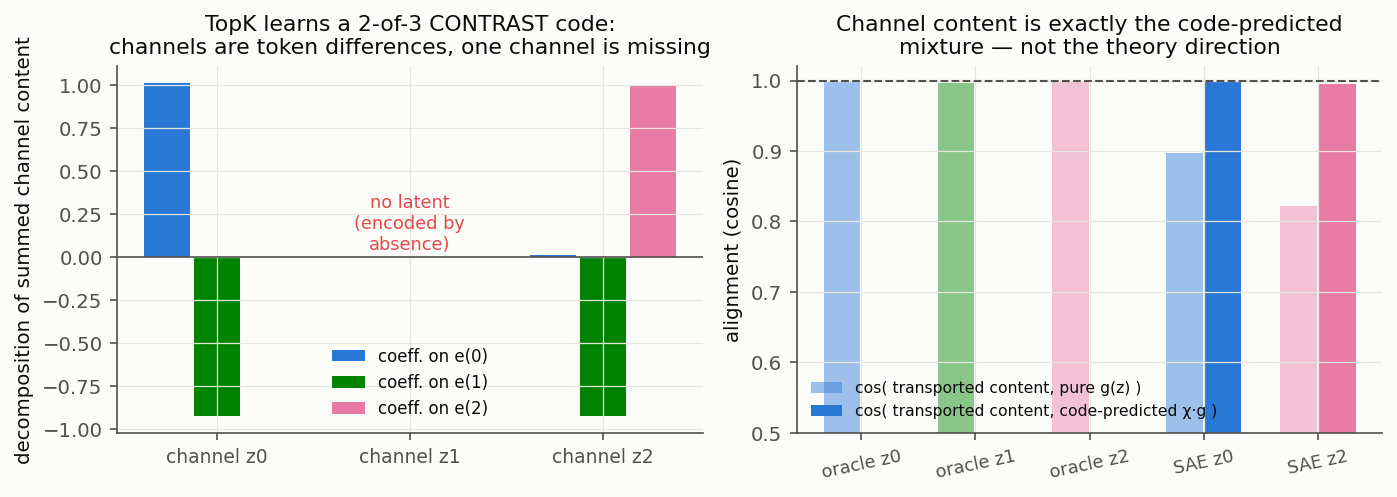
\includegraphics[width=0.86\textwidth]{../figures/dictionary.png}
\caption{\textbf{The learned code is a minimal contrast code.} A TopK SAE on
\texttt{resid\_pre} learns $9$ positional latents and $2$ token latents for
$3$ tokens; token 1 is encoded by \emph{absence}. The two token channels
decode as \emph{contrasts} against the absent token
($u_0\approx1.01\,e(0)-0.93\,e(1)$ and $u_2\approx1.00\,e(2)-0.93\,e(1)$),
not pure theory directions.}
\label{fig:dict}
\end{figure}

\subsection{Worked example: what TopK learned}

A TopK SAE ($12$ latents, $K=3$) on \texttt{resid\_pre} reconstructs to
$\mathrm{FVU}=2.3\times10^{-6}$ --- essentially perfect --- and (all three SAE
seeds agree) it partitions its latents as
\[
  \textbf{9 positional} \;+\; \textbf{2 token} \;+\; \textbf{1 dead}.
\]
Two token latents, for three tokens. The token-to-latent map is
$\{0\!\mapsto\!\{11\}\}$, $\{1\!\mapsto\!\{\,\}\}$, $\{2\!\mapsto\!\{5\}\}$:
\textbf{token 1 has no latent of its own.} It is encoded by absence --- when
neither token latent fires, the decoder bias supplies token 1. So ``sever token
1's channel'' is not an operation that exists in this latent set. (In the
oracle basis it exists and works: $\Delta\ceword=3.5\times10^{-3}$.) The
obstruction is the code's minimality, not the concept's reachability --- a
concrete instance of the rank-deficiency of single-feature cuts.

\subsection{The channels are contrasts, not directions}

Decode the summed token-0 channel back onto the token embeddings (least-squares
of its mean content on $[e(0),e(1),e(2),1]$ over the channel's support;
\texttt{dict\_deep.py}). Its token-content row is
\[
  \chi_0 = (\,1.012,\;-0.927,\;-0.000\,)\;\Longrightarrow\;
  u_0 \approx 1.01\,e(0)-0.93\,e(1),
\]
and token 2's is $\chi_2=(0.012,-0.926,1.000)$, i.e.\ $1.00\,e(2)-0.93\,e(1)$.
Both channels carry a $-0.93\,e(1)$ term: token 1, the absent one, is the shared
reference both contrasts subtract. So the channels do not transport pure
$\gv{z}$; they transport a \emph{mixture} $\chi_z\!\cdot\!\gv{}$. Check it
against the actual transported content (\texttt{dict\_deep.json}, verified with
both an independently-fit belief projector):
\begin{center}
\begin{tabular}{lrr}
\toprule
cosine of transported channel content with & token 0 & token 2 \\
\midrule
the code-predicted mixture $\chi_z\!\cdot\!\gv{}$ & $0.9992$ & $0.9953$ \\
the pure theory direction $\gv{z}$ & $0.90$ & $0.82$ \\
\bottomrule
\end{tabular}
\end{center}
The transported content matches the \emph{mixture} to cosine $0.999$, but is
$26^\circ$ off (cosine $0.90$) from the pure direction $\gv{0}$: about $27\%$ of
the channel's content ($\chi$-residual fraction $0.27$) is off-theory. If you
assumed ``SAE token-0 channel $=\gv{0}$'' you would edit along the wrong axis;
the code hands you a contrast, and you must extract the mixing matrix $\chi$
before your FRA edit means what you think.
(\emph{Honesty note, worth internalizing:} an earlier version of this script
estimated $\chi$ from an aliased cell-design regression and stored a mixture
cosine of $0.07$ --- badly wrong. The regenerated \texttt{dict\_deep.json} fits
$\chi$ cleanly over the channel's support and reports $0.9992$. The lesson is
exactly the section's: \emph{how you fit the code decides what the edit means}.)

\subsection{The intervention inherits the code}

This is not academic. Run the FRA-OV cut of token 0 \emph{through the SAE
channel} instead of the oracle direction. Because the channel is the contrast
$1.01\gv{0}-0.93\gv{1}$, cutting it does two things at once
(\texttt{ov\_edits.json}): it nulls token 0's tracking at
$c\approx0.54$ (predicted $c^\star=1/1.838$, Section~\ref{sec:rho}), \emph{and}
it \emph{boosts} token 1's tracking to $1.5\times$ at $c=1$ --- because the
channel's $-0.93\,e(1)$ component injects negative token-1 content, which reads
as more token-1 evidence once removed. The oracle cut and the SAE cut null the
same token at different gains and collateralize different neighbors: the edit
is exactly as clean as the code, and no cleaner.

\subsection{Purity does not see this}

Here is the sharp part. By the previous sprint's criterion --- set-level token
\emph{purity} --- these channels are perfect: $R^2\approx1.0000$, each token
latent fires on exactly its token. Purity is real and it is \emph{not
sufficient}. A channel can be perfectly pure and still be a contrast
($1.01\gv{0}-0.93\gv{1}$), still be missing entirely (token 1), still transport
a mixture. \textbf{What FRA edits actually inherit is the code's
\emph{completeness} and \emph{centering}}, and purity is blind to both. The one
diagnostic that would have caught it --- does the channel exist, and does its
transported content point where theory says --- is the mixing-matrix check
above, not the purity $R^2$.

One reassuring measurement to close the section: the deeper \texttt{resid\_mid}
SAE does \emph{not} hide the computation in its error term. Its reconstruction
error carries only $3.3\%$ of the belief-plane variance while being $5.9\%$ of
the total residual variance (\texttt{dict\_deep.json}): the error is
\emph{less} belief-laden than its size, so the SAE is not sweeping the belief
signal into the residual. When completeness and centering are good, FRA is
faithful; the failure mode is the code, not the method.

\fool{A clean purity table ($R^2=1.0$) reads as ``the SAE found the concept.''
It found a \emph{pure} code, which is necessary but says nothing about whether
the code is complete (token 1 is missing) or centered on theory directions (the
channels are contrasts). Trusting purity, you would cut ``token 0'' and silently
also inject token-1 content --- and your purity table would still say $1.0$.}

\section{Two heads, one truth}\label{sec:twohead}

\subsection{The question}

Everything so far was Config A, $\pzeta=+0.55$, one head. Flip to
\textbf{Config B}: $x=0.50$, so $\pzeta=1-3x=-0.50$. Now the process
\emph{anti}-correlates: even lags help, odd lags hurt. What does a single
softmax head do with a sign that flips every step --- and what happens to
per-head FRA attributions when the answer is ``it can't''?

\begin{figure}[t]
\centering
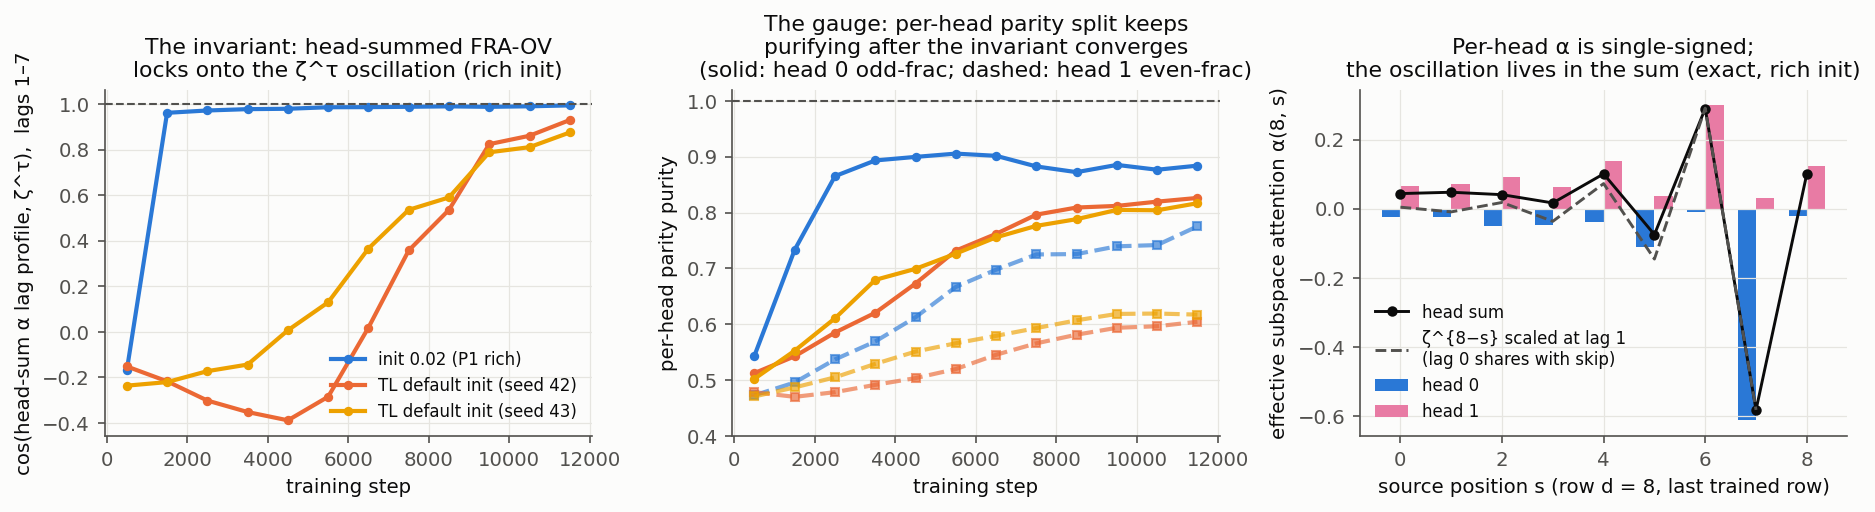
\includegraphics[width=\textwidth]{../figures/twohead.png}
\caption{\textbf{The two-head hinge at $\pzeta=-0.5$.} The head-summed effective
attention locks onto the signed $\pzeta^\tau$ oscillation as training proceeds
(cosine climbing), while the per-head parity split keeps drifting at nearly
constant loss. Rich (small) init converges the invariant faster than
TransformerLens-default init.}
\label{fig:twohead}
\end{figure}

\subsection{Why one head cannot: a one-line argument}

The target per-source coefficient is $\pzeta^{\,d-s}=(-1)^{d-s}|\pzeta|^{\,d-s}$
--- it alternates sign with lag. But a softmax attention row is a probability
distribution: \emph{every weight is non-negative}. A non-negative pattern times
a single OV direction cannot produce a sign that flips. So P2's solution is
forced: \textbf{two heads with anti-parallel OVs}. Head 1 (OV along $+\gv{}$)
carries the even lags; head 2 (OV along $-\gv{}$) carries the odd lags; the
head-\emph{sum} reproduces the oscillation,
\[
  \sum_{h=1,2}A^{(h)}_{d,s}f(v^{(h)}_s)
  = (-1)^{d-s}|\pzeta|^{\,d-s}\gv{z_s}=\pzeta^{\,d-s}\gv{z_s}.
\]

\subsection{Worked example: the oscillation lives only in the sum}

Take the last trained row ($d=8$) of our cleanest Config B checkpoint and read
off the per-head effective attention (\texttt{twohead.json}; formal note H1):
\begin{center}
\begin{tabular}{ll}
\toprule
head 0 coefficients $\alpha(8,\cdot)$ & \emph{all negative} (OV anti-parallel to $\gv{}$) \\
head 1 coefficients $\alpha(8,\cdot)$ & \emph{all positive} (OV parallel to $\gv{}$) \\
head-sum $\alpha(8,\cdot)$ & oscillates: $\dots,+0.29,\,-0.58,\,+0.10$ \\
theory $\pzeta^{\,8-s}$ & $\dots,+0.25,\,-0.50,\,+1.00$ \\
\midrule
$\cos(\text{head-sum},\,\pzeta^\tau)$, row-8 clean per-cell & $\mathbf{0.985}$ \\
\bottomrule
\end{tabular}
\end{center}
Neither head alone can carry the alternation --- each is single-signed. The
signed $\pzeta^{\,d-s}$ kernel appears \emph{only} in the sum, and there
(measured cell-by-cell on the clean row-8 pattern) it is recovered at cosine
$0.985$. \textbf{The head-sum is the invariant; the per-head split is not.}

\subsection{The invariant converges; the split never stops moving}

Track training (checkpoints every $500$ steps, \texttt{twohead.json}). The
head-sum's alignment with $\pzeta^\tau$ climbs and settles. On the lag-$1$--$7$
profile (the pinned tail, excluding the lag-0 term that the skip/diagonal split
depresses) our rich-init run goes from cosine $-0.17$ at step $500$ to
$\mathbf{0.994}$ by the end --- essentially exact. (The lag-0-included estimator
plateaus lower, at $0.72$, precisely because lag-0 content is shared with the
skip path; and the row-8 per-cell measurement above reads $0.985$. Same
invariant, three estimators.) Meanwhile the
\emph{per-head parity shares keep drifting} after the loss and the invariant
have both converged: head-1's even-lag fraction is still moving over the final
thousands of steps at essentially constant CE. The decomposition is a loss-flat
gauge coordinate; the sum is pinned.

\subsection{Rich vs.\ lazy init decides even the invariant}

One more wrinkle, the P2 App-G rich/lazy effect reproduced here (numbers on the
lag-0-included estimator, which resolves the init differences most sharply).
With small (``rich'') init the head-sum invariant converges smoothly
($0.23\to0.72$). With TransformerLens-default (``lazy'') init one seed's head-sum
cosine \emph{dips to $0.07$} mid-training before recovering to $0.63$ --- still
climbing at the end of P2's training budget --- while another default-init seed
reaches $0.75$. So even the \emph{invariant}'s convergence, not just the gauge
split, is init-dependent within a fixed budget. All seeds do pick the same canonical
even/odd parity assignment; they just get the sum sharp at different rates.

\keypoint{\textbf{Moral.} For $\pzeta<0$, per-head FRA-OV rankings are reads of a
\emph{gauge orbit} at a particular checkpoint and a particular init --- they
drift at constant loss and depend on initialization. Only the head-sum
$\sum_h A^{(h)}f(v^{(h)})=\pzeta^{\,d-s}\gv{z_s}$ is a trustworthy attribution.
\textbf{Sum the heads before you interpret.} A per-head bar chart is a snapshot
of a moving coordinate; the sum is the physics.}

\fool{A per-head attribution table at $\pzeta<0$ looks like a finding: ``head 1
does even lags, head 2 does odd.'' It is true \emph{at this checkpoint}, and it
keeps shifting while the loss sits still --- and a key-side cut applied at one
gain hits the two heads through \emph{different} normalizers, so it perturbs the
head-sum in a way that does not cancel. Read per-head numbers as gauge, never as
mechanism.}

\section{Coda: the factored world (Phase 2)}\label{sec:phase2}

Phase 2 moves to P1's \textbf{factored} process: two Mess3 components running in
parallel, $T=T^{(1)}\otimes T^{(2)}$, with their own eigenvalues $\pzeta_1,
\pzeta_2$ in two \emph{approximately orthogonal} $2$-dimensional residual
subspaces (three P1-faithful models, $100$k steps, all within $0.17$--$0.20$
millinats of Bayes). The whole apparatus of this note lifts per subspace: each
factor has its own update $\Delta r_n=\sum_s\pzeta_n^{\,d-s}\,g_n(z_s^{(n)})$,
and the FRA-OV attribution applies inside $V_{F_n}$. Two results are worth the
coda.

\begin{figure}[t]
\centering
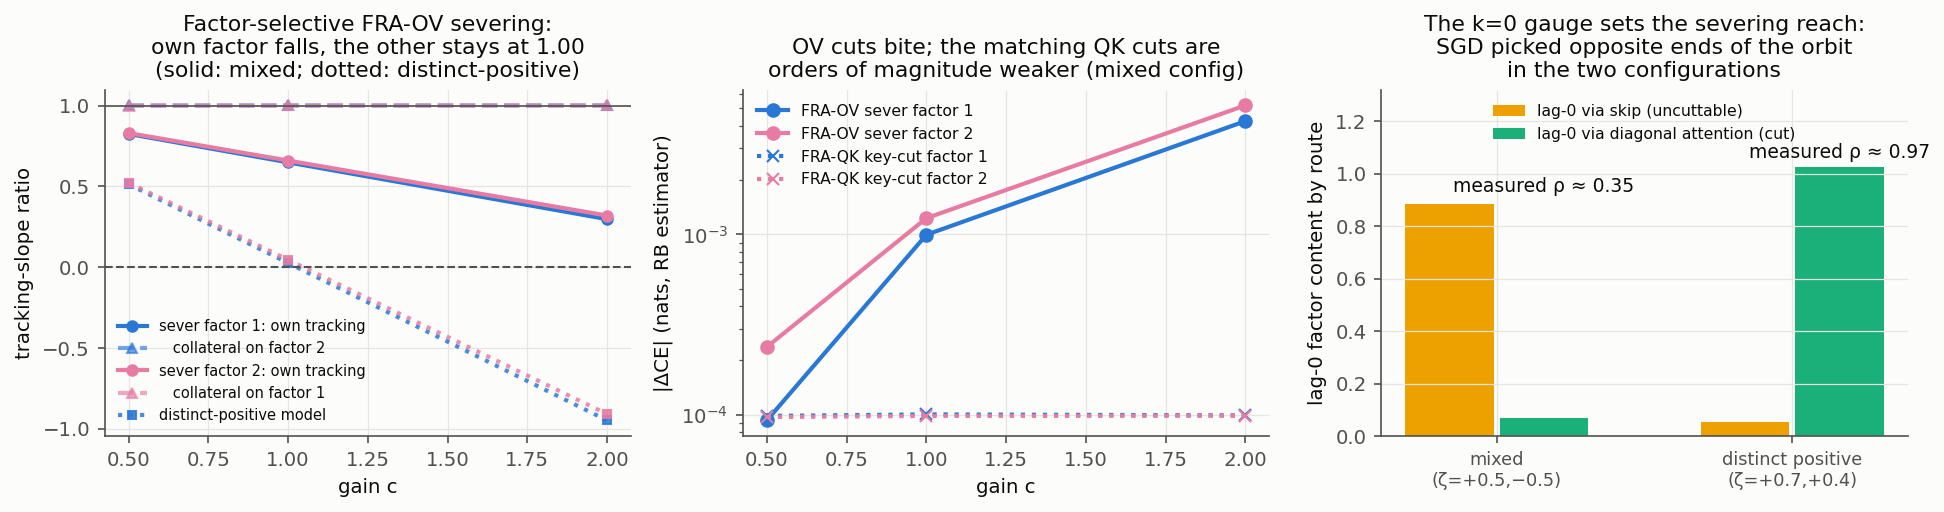
\includegraphics[width=\textwidth]{../figures/phase2_edits.png}
\caption{\textbf{Same cut, two runs, opposite reach --- and perfect cross-factor
protection.} Severing factor 1's OV channel severs $\rho\approx0.97$ per unit
gain in the distinct-positive model but only $\rho\approx0.35$ in the mixed
model (left) --- an inter-model instance of Phase~1's $c^\star=1/\rho$ gauge law.
Cross-factor tracking (right) stays at $+1.00$ at every gain in every model:
orthogonal subspaces mean no forced collateral, unlike Mess3's $1.5\times$.}
\label{fig:phase2}
\end{figure}

\textbf{Both eigenvalues from one model, and a dead head you can see in one
number.} The per-factor effective subspace attention recovers each factor's
$\pzeta_n$ from a \emph{single} trained model: distinct-positive ($\pzeta=
(0.7,0.4)$) gives lag-ratios $0.705$ / $0.381$ (cosine with $\pzeta_n^\tau$
$0.997$ / $0.9995$); mixed ($\pzeta=(0.5,-0.5)$) gives $0.572$ / $-0.570$ vs
$\pm0.5$, the sign oscillation living only in the head-sum as in
Section~\ref{sec:twohead}. How heads divide the labor is itself a finding: the
distinct-positive model \emph{specializes} (head-factor share matrix
$\genfrac[]{0pt}{1}{0.95\ 0.28}{0.05\ 0.72}$, one head per factor), the mixed
model \emph{collaborates} ($\genfrac[]{0pt}{1}{0.64\ 0.64}{0.36\ 0.36}$, roles
split by parity not factor). And in the three-head mixed model the third head
carries share $0.0005$ / $0.00006$ of the two factors --- \textbf{a dead head},
P1's conic minimum-head-count $H_{\min}=2$ with ray reuse, visible in one
number.

\textbf{Cross-factor collateral is exactly zero --- the prediction from
Section~\ref{sec:ov} confirmed.} In P2's single Mess3 selective removal was
impossible because the three $\gv{z}$ share one $2$-plane. Here the factors live
in orthogonal subspaces, so severing factor $n$ should leave factor $m$
untouched --- and it does, to the digit: factor $m$'s tracking sits at $+1.00$ at
\emph{every} gain in \emph{every} model (Fig.~\ref{fig:phase2}, right), against
Mess3's geometrically forced $1.5\times$. FRA-QK factor cuts stay inert
($-1$ to $-3.4\times10^{-4}$ nats, gain-independent, tracking $1.00$); FRA-OV
cuts reach $1.5\times10^{-2}$ nats and null tracking --- the same QK-gauge /
OV-handle split as Phase~1, now per factor.

\textbf{The teaching-gold: the spectrum, not luck, picks the severing reach.}
The two headline slopes --- distinct-positive severs $\rho\approx0.97$ (null at
$c\approx1.03$), mixed severs only $\rho\approx0.35$ --- come from the
\emph{same} OV cut on the \emph{same} task family. What differs is not the
embedding (the token$\times$position interaction share is $1.1\%$ in both; we
tested and refuted the ``one model factored its embeddings better'' hypothesis
first). It is the $k{=}0$ gauge of Section~\ref{sec:ov}, now varying
\emph{across models}: the distinct-positive run delivers its lag-0 factor
content through \emph{diagonal attention} (the $\alpha$ lag-0 coefficient is
$0.96$), so an OV cut catches it; the mixed run delivers the same content
through the \emph{skip} ($\alpha$ lag-0 coefficient $0.05$), so an OV cut misses
it --- and at $|\pzeta|=0.5$ that lag-0 term is about half the evidence. And
which end of the orbit a model lands on is \emph{not} seed luck: across six
models spanning both phases, seeds, and init scales, every positive-spectrum
config sits at the diagonal end and every config carrying a negative eigenvalue
sits at the skip end (the seed-43 replicas land exactly where their seed-42
twins did). The \emph{data's spectrum} picks the end of the gauge orbit, not
SGD's coin. Phase~1 warned that ``$c^\star$ is a property of the run, not the
task'' (the $\rho(a_0)$ sweep, Section~\ref{sec:ov}); Phase~2 sharpens it --- the
run's gauge position is itself a systematic function of the spectrum. Read a
severing gain as a fact about the model's spectrum and gauge, never about the
concept.

\textbf{And the dictionary lesson recurs.} The P1-world SAE learns a complete
per-value code for the positive factor (three latents) but gives the
\emph{negative} factor a single latent for its three values ($11/24$ latents
mixed, FVU $7.5\times10^{-3}$) --- the completeness gap of
Section~\ref{sec:dict}, and it selects against exactly the factor whose content
is split across anti-parallel heads. The binding constraint is, again, the
code.

\fool{You might notice that these Phase-2 rates ($0.705/0.381$) sit at the
\emph{raw} eigenvalues $\pzeta=(0.7,0.4)$, not the shrunk optima of
Section~\ref{sec:ladder} --- and conclude the shrinkage story was P2-specific.
It was not: the per-factor MSE-optimal rates \emph{are} shrunk, to
$\eta^\star=0.60/0.34$ (the same $0.85$ factor that gave $0.464$ in P2), but
moving from $\eta^\star$ to raw $\pzeta$ costs only $2.2\%$ / $0.56\%$ of each
factor's (already microNat) lag-information. The \emph{rate itself} is loss-flat
--- Section~\ref{sec:ladder}'s mechanism applied to the decay parameter rather
than the tail values --- so SGD sits at raw $\pzeta$ with no pressure to shrink.
(Likewise the product process carries a third eigenvalue $\pzeta_1\pzeta_2=0.28$,
the $g_1\!\otimes\!g_2$ cross term of the displacement: its optimal geometric is
real but worth $\sim2\times10^{-5}$ nats --- present in the theory, invisible to
the trained model. Loss-flatness is not one finding; it is the weather of this
whole world.)}

\section{Field guide: five questions before you trust an FRA reading}\label{sec:guide}

Everything above compresses to a checklist. Before attributing anything to a
feature-resolved attention number, run these five.

\keypoint{
\textbf{1. Is the structure loss-pinned?} Compute (or estimate) the CE value of
the lag, row, or window you are reading. If the loss never paid for it --- the
geometric tail, the gradient-free last row (Section~\ref{sec:ladder}) --- your
``mechanism'' is seed noise. In this world, only lags $0$--$2$ and rows $1$--$8$
were pinned; everything else was free.

\smallskip
\textbf{2. Is the coefficient a gauge coordinate? Dial it.} FRA-QK cut effects
are dialable across $140\times$ at bit-identical behavior by a loss-preserving
re-split (Section~\ref{sec:dial}). Before reporting a score attribution, apply
the gauge move and watch whether your number survives. If it can be sent to
zero, it was a coordinate, not a computation.

\smallskip
\textbf{3. Is the channel complete and centered?} An SAE channel can be
perfectly \emph{pure} ($R^2=1$) and still be a \emph{contrast}
($1.01\gv{0}-0.93\gv{1}$), or missing entirely (token 1 has no channel;
Section~\ref{sec:dict}). Extract the mixing matrix $\chi$ and check the
transported content points where theory says --- purity will not tell you.

\smallskip
\textbf{4. Did you sum the heads?} For $\pzeta<0$, per-head attributions drift
at constant loss and depend on init (Section~\ref{sec:twohead}). Only the
head-sum is the invariant. Sum before you interpret; a per-head bar chart is a
snapshot of a moving coordinate.

\smallskip
\textbf{5. Can your edit even be surgical here?} Count dimensions. If the concept
directions span fewer dimensions than there are directions (2 vs 3 in Mess3),
selective removal is geometrically impossible and \emph{all} of your collateral
is forced, independent of method (Section~\ref{sec:ov}). Know this before you
blame your SAE.
}

\medskip
The through-line: FRA-QK measures gauge, FRA-OV measures a real (but
non-surgical) handle, and both are exactly as trustworthy as your answers to
questions 1--5. In a $9.4$-millinat world where every quantity has a closed
form, we could check each answer against the ground truth. On a real model you
cannot --- which is precisely why the checklist, and not any single number, is
the thing to carry over.

\end{document}
